\subsection{damBreak}\label{header-n531}

Colapso de una columna de agua en un tanque que representa la rompiente
contra un dique, como ya se ha mencionado se trata de un tutorial de
OpenFOAM \cite{dambreak}, ubicado en
\lstinline[style=bash]{$FOAM_RUN/tutorials/multiphase/interFoam/laminar}.

\subsubsection{Definición del caso}\label{header-n536}

\begin{itemize}
\item
  Objetivos planteados:

  \begin{itemize}
  \item
    Simular la caida de una columna de agua, la cual choca contra un
    obstáculo (colocado en la parte central de la base) lo
    suficientemente pequeño como para que el volumen de agua lo
    sobrepase y golpee contra las paredes de un tanque hasta su
    estabilización.
  \item
    Analizar el comportamiento de la Superficie Libre de Líquido (SLL),
    para ello se prestará especial atención al cálculo de la fracción de
    volumen relativo a las dos fases del flujo en cada celda.
  \end{itemize}
\item
  Condiciones iniciales:

  \begin{itemize}
  \item
    Caso en 2D, multifásico, laminar, incompresible, Newtoniano. \\
  \item
    Mediante la aplicación \textbf{``interFoam''} se resuelven las
    ecuaciones de RANS (Reynold-average Navier-Stokes) para dos fases
    inmiscibles de flujos y se consigue monitorizar el movimiento de la
    SLL usando la técnica de Volúmenes Finitos (\emph{Volume of Fluid},
    VOF).
  \item
    La discretización de las ecuaciones se lleva a cabo con el método MULES\footnote{\url{http://www.openfoam.org/version2.3.0/multiphase.php}}
    (Multidimensional Universal Limiter with Explicit Solution) creado
    por OpenCFD, donde se resuelve la Ecuación de Transporte,
    determinando la fracción de volumen relativo a las dos fases, o
    \textbf{fracción de fase}, en cada celda (estableciendo como
    condición inicial para la fracción de fase 1 para la fase de agua y
    0 para la fase del aire).
  \item
    Abierto a la atmosfera, permitiendo la entrada y salida del flujo de
    aire. Usando el método de acoplamiento \textbf{PIMPLE}, se
    implementa una combinación de condiciones para hallar la presión y
    la velocidad y se resuelve simultáneamente la continuidad y
    conservación de momento.
  \end{itemize}
\item
  Condiciones de contorno:

  \begin{itemize}
  \item
    Las condiciones de contorno se determinan para \emph{leftWall,
    rightWall, lowerWall, atmosphere} y \emph{defaultFaces}.
  \item
    Se especifica el tipo \emph{zeroGradient} a las paredes; y como está
    abierto a la atmósfera se emplean las condiciones
    \emph{totalPressure, inletOutlet} y
    \emph{pressureInletOutletVelocity}.
  \end{itemize}
\item
  Propiedades físicas y fuerzas exteriores

  \begin{itemize}
  \item
    Para el agua se establece una \emph{viscosidad cinemática (nu)} de
    \(1\times10^{-6} m^2/s\) y una \emph{densidad (rho)} de
    \(1000 kg/m^3\).
  \item
    En cambio, el aire se define con una \(\nu=1,48 \times ^{-5} m^2/s\)
    y una \(\rho=1kg/m^3\).
  \item
    Como fuerza exterior se define la gravedad, con un valor en \emph{y}
    de \(g=-9,81m/s^2\).
  \end{itemize}
\item
  Modelo de turbulencia:

  \begin{itemize}
  \item
    Laminar, sin turbulencia.
  \item
    También se ejecutó el caso para implementar la turbulencia del tipo
    RAS, disponible entre los ejemplos de OpenFOAM v4, con el modelo
    \(k-\epsilon\) (\emph{kEpsilon}).
  \end{itemize}
\item
  Esquema de discretización:

  \begin{itemize}
  \item
    El esquema de discretización para la primera derivada del tiempo
    \texttt{ddtSchemes}: \textbf{Euler}, adecuado para problemas
    transitorios, implícito de primer orden, estable.
  \item
    El siguiente subdiccionario \lstinline[style=bash]{gradSchemes} contiene los
    términos gradientes. Se emplea el esquema de discretización más
    común: \textbf{Gauss linear}, esta entrada especifica la
    discretización estandar de volúmenes finitos, la integración
    Gaussiana, la cual requiere la interpolación de los valores
    centrados en las celdas a los centrados en las caras.
  \item
    El subdiccionario \lstinline[style=bash]{divSchemes} contiene los términos
    divergentes. El tratamiento de los términos advectivos es uno de los
    mayores retos en CFD numérico y por ello las opciones son más
    extensas. La forma más usual de los términos advectivos suele ser
    \texttt{div(phi,...)}, donde \emph{phi} indica generalmente el flujo
    (volumétrico) de velocidad en las caras de las celdas, para flujos
    de densidad constante y el flujo másico para flujos compresibles,
    por ejemplo \texttt{div(phi,U)} para la advección de la velocidad,
    \texttt{div(phi,k)} para la energía cinética de la turbulencia, etc.
  \item
    El subdiccionario \texttt{laplacianSchemes} contiene términos de
    Laplace. Por ejemplo, el término de difusión de la ecuación del
    momento, el cual se corresponde con \texttt{laplacian(nu,U)}. El
    esquema de Gauss es la única opción para la discretización y
    requiere una selección tanto de un esquema de interpolación para el
    coeficiente de difusión, viscosidad, como de un esquema del
    gradiente de la normal a la superficie.
  \end{itemize}
\item
  Procedimiento de resolución:

  \begin{itemize}
  \item
    Para cada una de las variables (p y U) se define el tipo de
    resolvedor, junto con los parámetros necesarios. El utilizado para
    la \emph{p} y la \emph{U} es: \textbf{PCG} (\emph{preconditioned
    conjugate gradient}), para matrices simétricas.
  \item
    Por otro lado, el precondicionamiento de las matrices viene dado por
    \textbf{DIC} (\emph{diagonal incomplete-Cholesky}), para matrices
    simétricas.
  \item
    Para la fracción de fase se especifica un suavizado
    \texttt{smoothSolver} del tipo \texttt{symGaussSeidel}.
  \end{itemize}

  Además se usa \textbf{PIMPLE}, versión mejorada de PISO
  (\emph{Pressure Implicit with Splitting of Operators}), combinado con
  SIMPLE (\emph{Semi-Implicit Method for Pressure- Linked Equations}),
  permite garantizar la convergencia de las ecuaciones en cada paso del
  tiempo.
\item
  Control del paso del tiempo:

  Cuando se presenta en un caso la condición de capa libre, el
  algorítmos es considerablemente más sensible al número de Courant,
  para este caso el máximo valor de \texttt{maxCo} se fija en 1. Donde
  la propagación de la velocidad sea difícil de predecir, se especifica
  un paso del tiempo más ajustado, además, \emph{interFoam} ofrece un
  ajuste automático de un paso de tiempo predeterminado
  \texttt{adjustableRunTime}. Aparte de esto, los valores que
  determinarán el guardado de la solución son:

  \begin{itemize}
  \item
    Tiempo de simulación: de 0 a 5 segundos.
  \item
    Paso del tiempo: 0,001.
  \item
    Intervalo de escritura: 0,025.
  \end{itemize}
\end{itemize}

\subsubsection{Ejecución del caso}\label{header-n645}

Los pasos para ejecutar este caso son:

\begin{figure}[hb]
\centering
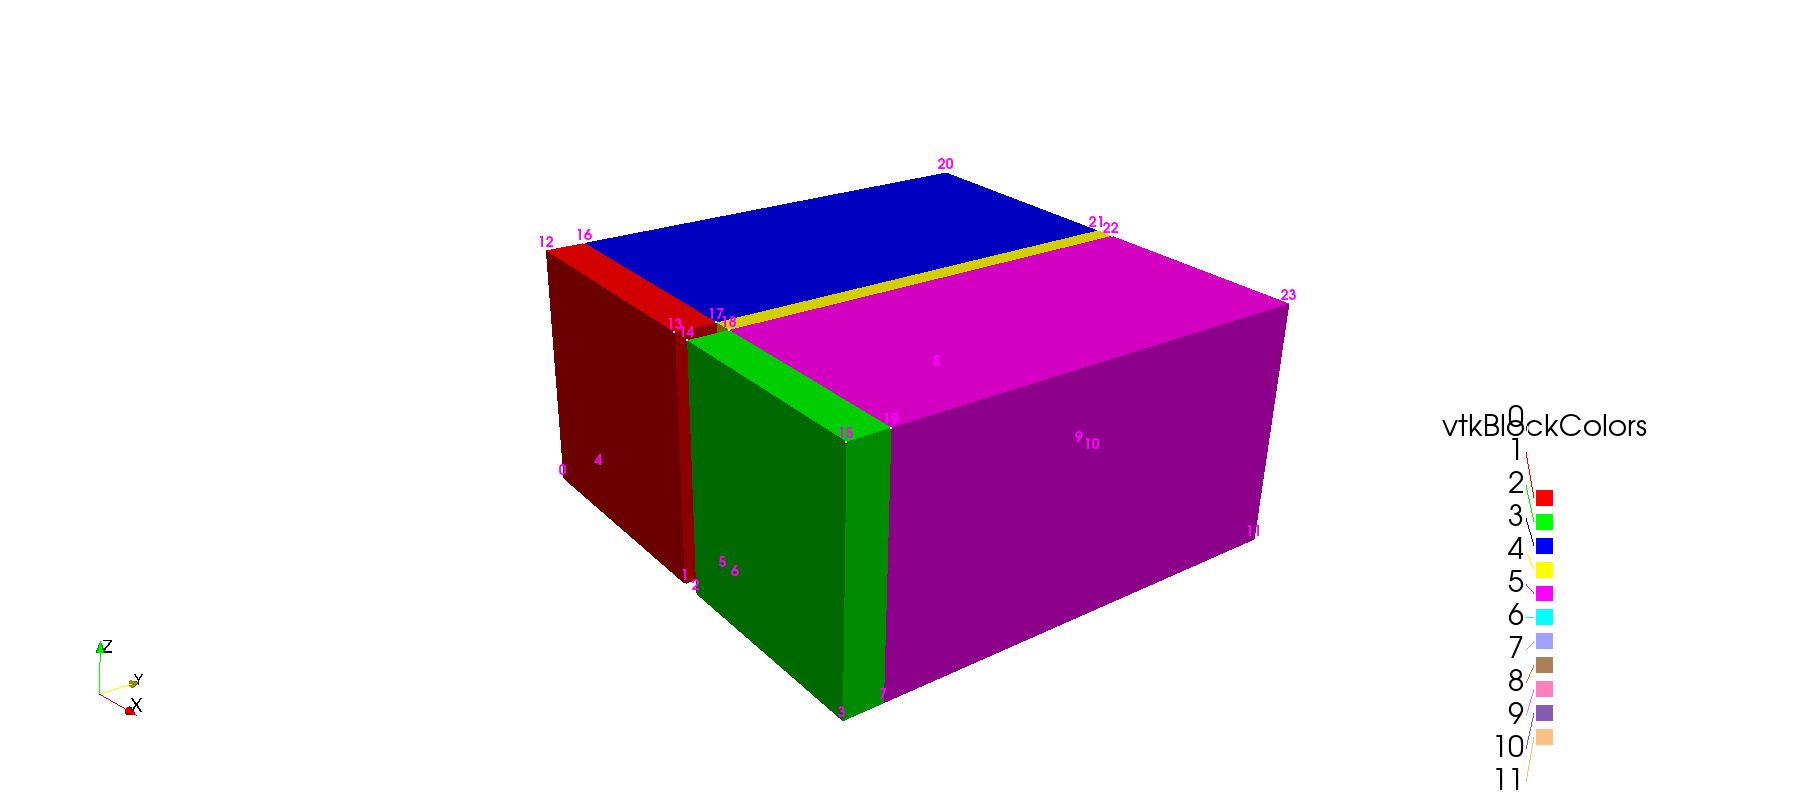
\includegraphics[width=\linewidth]{bMvertex.png}
\caption{Bloque del modelo con los vértices enumerados}
\label{fig:bMvertex}
\end{figure}

\begin{enumerate}
\def\labelenumi{\arabic{enumi}.}
\item
  Desde la ubicación del caso, introducir la orden: \texttt{blockMesh}.
  La cual genera los ficheros \emph{boundary, faces, neighbour, owner} y
  \emph{points}, que definen el modelo (geometría y mallado) en
  \lstinline[style=bash]{./constant/polyMesh\textgreater}. Para visualizar estos
  resultados, ejecutar \texttt{paraFoam} y para mostrar los bloques del
  modelo se puede utilizar la orden: \texttt{paraFoam\ -block}, el resultado se puede ver el \autoref{fig:bMvertex}.



  \textbf{NOTA}: Esta orden implicará volver a ejecutar
  \texttt{blockMesh}, ya que los ficheros generados son eliminados.
\item
  La definición de la condición inicial del agua se da mediante la orden
  \texttt{setFields}, pero antes, se debe comprobar que en la carpeta
  \lstinline[style=bash]{./0} existan dos ficheros: \emph{alpha.water}
  y \emph{alpha.water.orig}. El segundo, corresponde a una copia de
  seguridad, puesto que, al ejecutar \texttt{setFields} se reescribe el
  fichero para definir la fracción de volumen por cada celda.

  En caso de querer volver a ejecutar el caso, eliminar el contenido de
  \emph{alpha.water} y copiar el de \emph{alpha.water.orig} en el mismo.
  También se puede realizar esta acción, introduciendo la orden:
  \lstinline[style=bash]{cp 0/alpha.water.orig 0/alpha.water}.
\item
  Procesar el caso introduciendo la orden \texttt{interFoam}. Se puede
  añadir el argumento \lstinline[style=bash]{interFoam > log.interFoam}
  para ejecutar la orden y registrar la solución en el fichero
  ``\emph{log.application}'' (también funciona para las órdenes
  anteriormente mencionadas). Asimismo, la orden
  \lstinline[style=bash]{interFoam | tee log.interFoam} permite visualizar
  los resultados por terminal además de guardarlos. Por último, si el
  caso ya ha sido ejecutado y terminado, pero se quiere volver a
  ejecutar, guardando los resultados a continuación de los anteriores,
  se añade el argumento \emph{-a} en la orden:
  \lstinline[style=bash]{interFoam | tee -a log.interFoam}, de este modo,
  el programa sabrá que el archivo donde se registrará la solución ya
  existe. La visualización del caso se puede apreciar en \autoref{fig:damBreak}.
\end{enumerate}

\begin{figure}[hb]
\centering
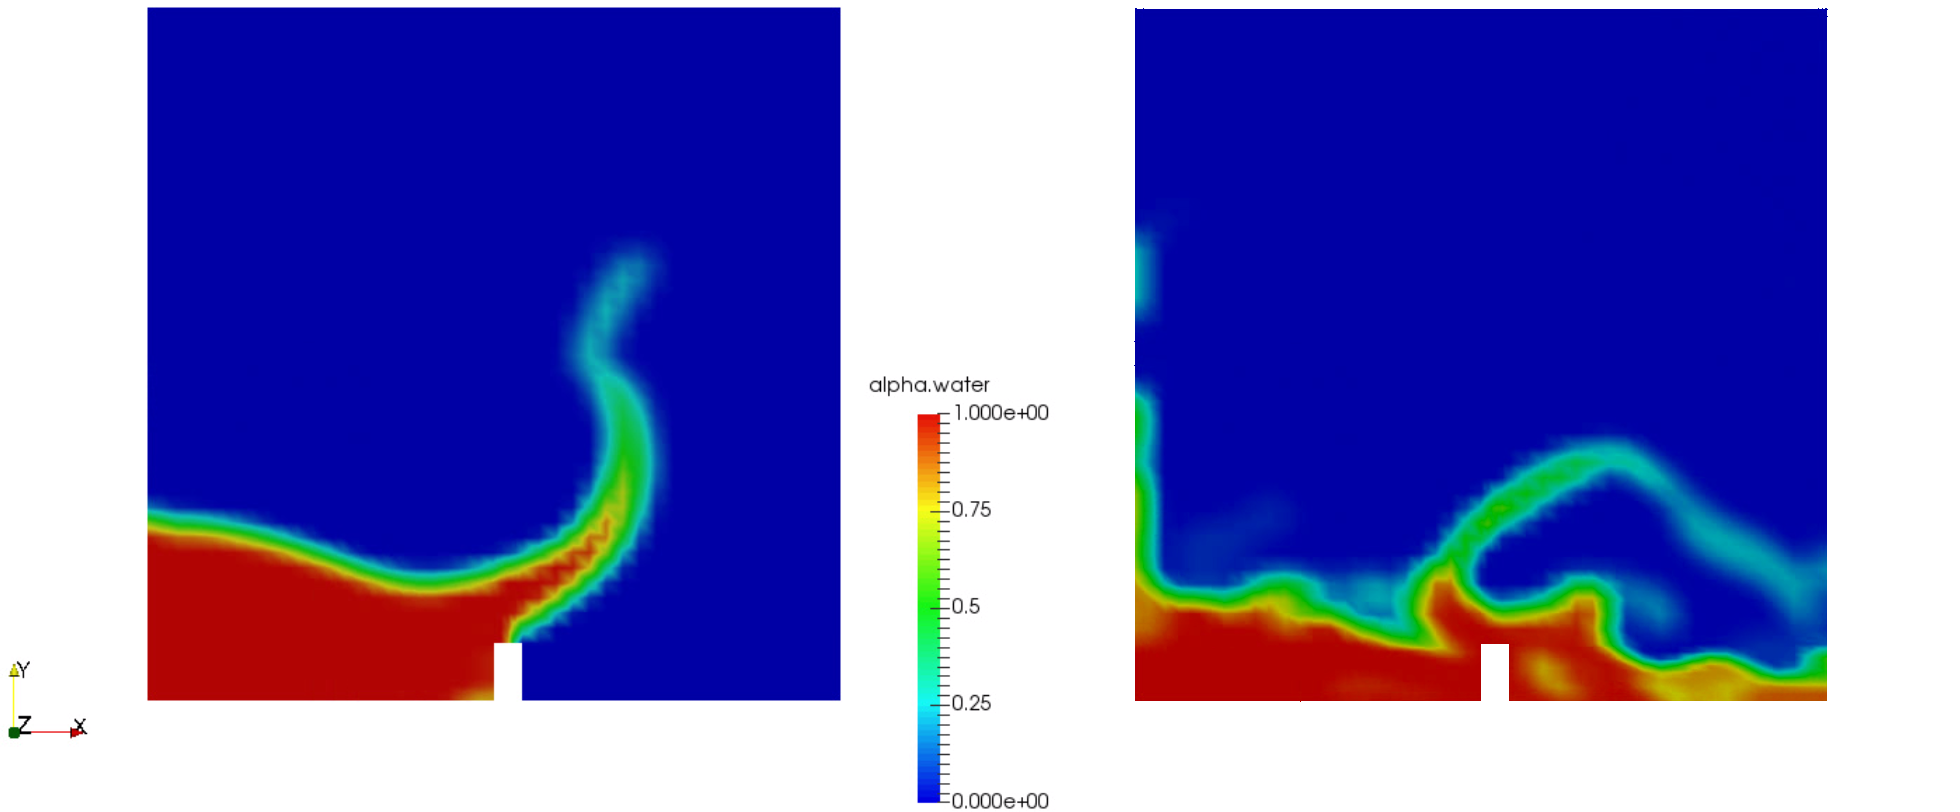
\includegraphics[width=\linewidth]{damBreak.png}
\caption[Animación del caso]{Imágenes de la ejecución del caso, obtenidas desde ParaView}
\label{fig:damBreak}
\end{figure}

\subsection{damBreakFine}\label{header-n674}

Se trata de una continuación del caso anterior, mostrando cómo aumentar
la resolución de la malla y ejecutar el caso en paralelo. La información
detallada sobre las ejecuciones de los casos en paralelo, se dan en \emph{User
Guide: 3.4 Running applications in parallel}\footnote{\url{http://cfd.direct/openfoam/user-guide/running-applications-parallel}}.

\subsubsection{Definición del caso}\label{header-n679}

\begin{itemize}
\item
  Objetivos planteados:

  \begin{itemize}
  \item
    Realizar cambios en la geometría del mallado desde el directorio
    \lstinline[style=bash]{./constant/polyMesh/blockMeshDict}.
    Modificando el \emph{radio de expansión}
    \lstinline[style=c++]{simpleGrading (1 2 1)}, hace que se refine el fondo,
    disminuyendo el tamaño de celdas a la mitad en proporción a las
    celdas superiores en el eje \emph{y}.
  \item
    Correr el caso en paralelo.
  \end{itemize}
\item
  Condiciones iniciales:

  \begin{itemize}
  \item
    La velocidad y la presión se mantienen uniformes, ya que son
    independientes del número de elementos por capa.
  \end{itemize}
\item
  Control de la solución:

  \begin{itemize}
  \item
    En este tutorial, el método de descomposición del dominio es
    \texttt{simple} y los coeficientes (\emph{SimpleCoeff}) deben
    editarse en base a los siguientes critérios:

    \begin{itemize}
    \item
      El número de subdominios a especificar (en \emph{x, y, z}) suele
      corresponder con el número de procesadores disponibles.
    \item
      Aunque también se puede determinar en función del dominio, como es
      el caso, donde el número de subdominios se define con el vector
      \textbf{n}.
    \item
      Como se trata de una geometría bidimensional, en la dirección
      \emph{z}, no se divide el dominio, por tanto, \(nz=1\).
    \item
      Será beneficioso conservar el número de celdas por caras
      colindante con la descomposición, por ello, para una
      descomposición cúbica, es recomendable mantener la división en las
      direcciones \emph{x} e \emph{y} equitativa. Es decir,
      \(n_xn_y= \text{numberOfSubdomains}\).
    \end{itemize}
  \end{itemize}
\end{itemize}

\subsubsection{Ejecución del caso}\label{header-n720}

\begin{figure}[ht]
\centering
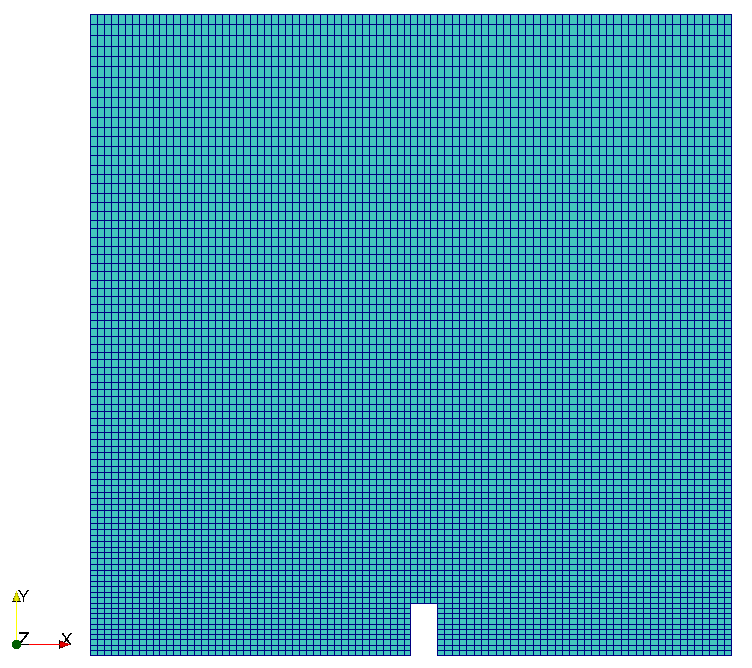
\includegraphics[scale=0.40]{mesh-damBreakFine.png}
\caption{Mallado del caso con blockMesh}
\label{fig:mesh-damBreakFine}
\end{figure}

\begin{enumerate}
\def\labelenumi{\arabic{enumi}.}
\item
  Modificar el \emph{radio de expansión}
  \lstinline[style=c++]{simpleGrading (1 2 1)}, lo que hace que se refine el fondo,
  disminuyendo el tamaño de celdas a la mitad en proporción a las celdas
  superiores en el eje \emph{y}. Ejecutar \texttt{blockMesh} para generar la
  malla definida, pudiendo visualizarla a través de ParaView \autoref{fig:mesh-damBreakFine}.

\item
  Comprobar que la malla no de errores: \texttt{checkMesh}.
\item
  Reinicializar la fase \emph{alpha.water}:
  \lstinline[style=bash]{cp 0/alpha.water.orig 0/alpha.water} y ejecutar
  \texttt{setFields}. Las variables \emph{U} y \emph{$p_rgh$} son
  independientes de los cambios en el mallado, ya que se especifican
  como valores uniformes.
\item
  Se emplea la utilidad de \texttt{descomposePar}, para descomponer el
  dominio. Como otras utilidades de OpenFOAM, se puede encontrar el
  directorio asociado en el código fuente
  \lstinline[style=bash]{$FOAM\_UTILITIES/parallelProcessing/decomposePar}.
  En este caso, se ejecuta con 4 procesadores (o
  \emph{numberOfSubdomains}), luego \emph{n= (2 2 1)} y la entrada
  \emph{delta} debe establecerse en 0,001.
\item
  El caso muestra un ejemplo de ejecución en paralelo, donde se utiliza
  la implementación \emph{openMPI} de interfaz estándar de traspaso de
  información (\emph{message-passing interface}, MPI). La siguiente
  orden, permite al usuario ejecutar el caso en paralelo, en un solo
  nodo (el ordenador local solamente):

  \lstinline[style=bash]{mpirun -np 4 interFoam -parallel > log &}.
\item
  Por ultimo se revierte el proceso de descomposición mediante la orden:
  \texttt{reconstructPar}
\end{enumerate}

\begin{figure}[ht]
\centering
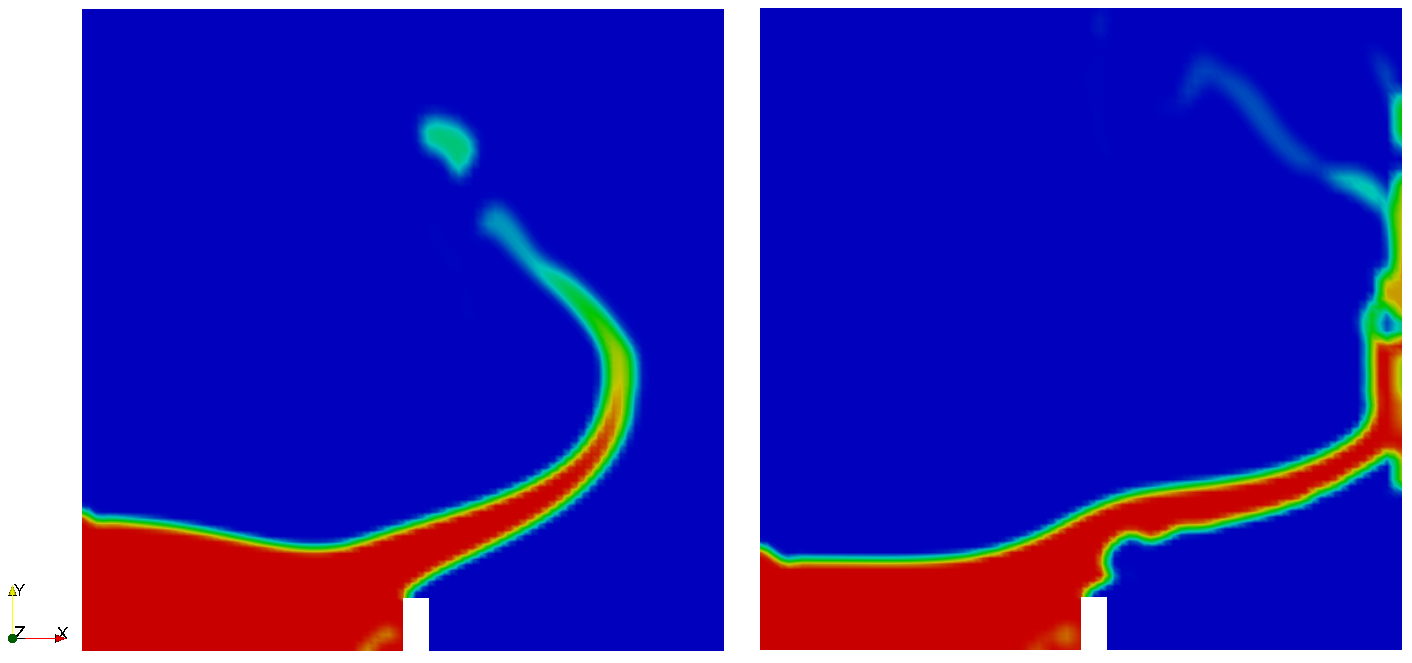
\includegraphics[width=\linewidth]{damBreakFine.png}
\caption{Imágenes de la ejecución del caso, ParaView}
\label{fig:damBreakFine}
\end{figure}

\subsection{damBreakMod}\label{header-n750}

En este caso, se modifican los vértices del modelo desde el fichero
blockMeshDict y se añade un nuevo contorno, para asemejar el modelo al
principio de captación de energía OWC. Además se añade la turbulencia
del caso ejemplo:

\lstinline[style=bash]{$FOAM_run/tutorials/multiphase/interFoam/RAS/damBreak}.

Se recomienda partir por este caso ya que, la adición de la turbulencia,
conlleva cambios en el esquema de discretización y en el procedimiento
para alcanzar la solución.

\subsubsection{Definición del caso}\label{header-n755}

\begin{itemize}
\item
  Objetivos planteados:

  \begin{itemize}
  \item
    Comenzar a realizar cambios en la geometría que permitan ir viendo
    como llegar a la solución final.
  \item
    Implementar el modelo de turbulencia \(k-\epsilon\), para observar
    los cambios en la representación del movimiento del flujo.
  \item
    Aumentar el volumen inicial de agua, ya que se necesita representar
    una columna oscilante de agua en la parte de la cámara (representada
    a la derecha, abierta por el fondo).
  \end{itemize}
\item
  Modelo del caso:

  \begin{itemize}
  \item
    Se modifica y se añaden vértices a mano desde el diccionario
    dedicado para ello \lstinline[style=bash]{./system/blockMeshDict},
    esto implicará la adición de nuevos bloques y variar la composición
    de algunos contornos. Las dimensiones se calculan como múltiplos de
    la anchura de las celdas. Se pueden comparar los cambios con el caso
    original, mediante alguna herramienta diseñada para ello, para este
    caso se utiliza: \lstinline[style=bash]{meld damBreak damBreakMod}.
  \end{itemize}
\item
  Condiciones iniciales:

  \begin{itemize}
  \item
    La condición inicial del agua, se define en
    \lstinline[style=bash]{./system/setFieldsDict}, detallado en el
    tutorial de \emph{damBreak}. En este caso, la función \texttt{boxToCell}
    crea un volumen delimitado por un vector mínimo (0 0 -1) y otro
    máximo (1.75 2 1) que definen la diagonal del prisma, para definir
    el conjunto de celdas que corresponda a la región del agua (la
    fracción de fase del agua se define como \(\alpha=1\)).
  \item
    La adición del modelo de turbulencia implicará definir las
    siguientes variables en la carpeta \lstinline[style=bash]{./0}:
    \emph{epsilon, k, nut} y \emph{nuTilda}. Extraidas del ejemplo de
    tutorial
    \lstinline[style=bash]{\$FOAM\_run/multiphase/interFoam/ras/damBreak\textgreater}.
  \end{itemize}
\item
  Condiciones de contorno:

  \begin{itemize}
  \item
    Dentro del diccionario
    \lstinline[style=bash]{./system/blockMeshDict}, se añade un nuevo
    contorno \emph{topWall}, en la parte derecha donde se representa una
    cámara, por el momento cerrada a la atmósfera.
  \end{itemize}
\item
  Modelo de turbulencia:

  \begin{itemize}
  \item
    Ubicado en \lstinline[style=bash]{./constant/turbulenceProperties},
    para el tipo de simulación RAS se define el modelo \emph{kEpsilon} y
    se activa la turbulencia, así como la escritura de los coeficientes.
  \end{itemize}
\item
  Esquema de discretización:

  \begin{itemize}
  \item
    Se añade el esquema para la divergencia para las variables añadidas
    por la turbulencia:

\begin{lstlisting}[style=c++]
div(phi,k)      Gauss upwind;
div(phi,epsilon) Gauss upwind;
\end{lstlisting}
  \end{itemize}
\item
  Procedimiento para la solución:

  \begin{itemize}
  \item
    De forma análoga al punto anterior, se incluyen las variables para
    la solución, dentro de los mismos parámetros establecidos para la
    velocidad \emph{U}, con la adición de la última línea:

\begin{lstlisting}[style=c++]
"(U|k|epsilon).*"
{
    solver          smoothSolver;
    smoother        symGaussSeidel;
    tolerance       1e-06;
    relTol          0;
    minIter         1;
}
\end{lstlisting}
  \end{itemize}
\end{itemize}

\subsubsection{Ejecución del caso}\label{header-n819}

\begin{figure}
\centering
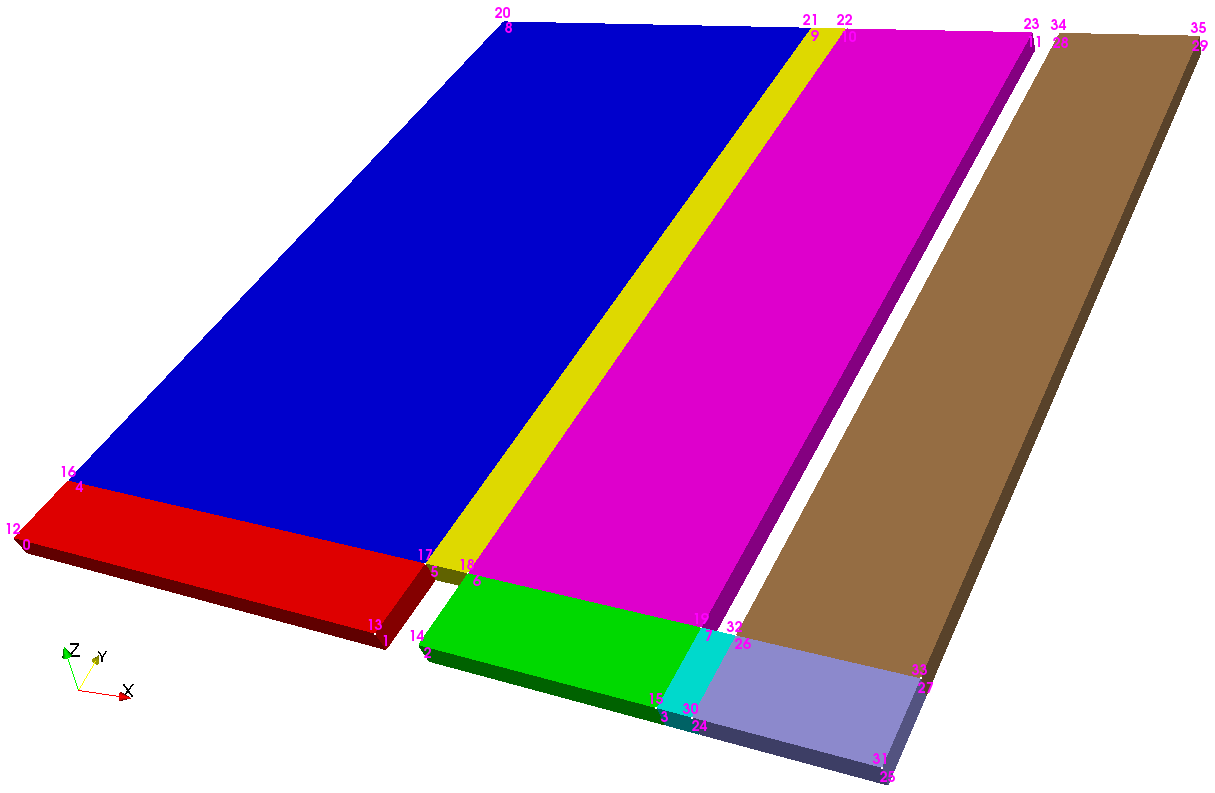
\includegraphics[width=\linewidth]{blockdanmBreakMod.png}
\caption{Bloques y vértices del modelo del caso}
\label{fig:blockdanmBreakMod}
\end{figure}

\begin{figure}
\centering
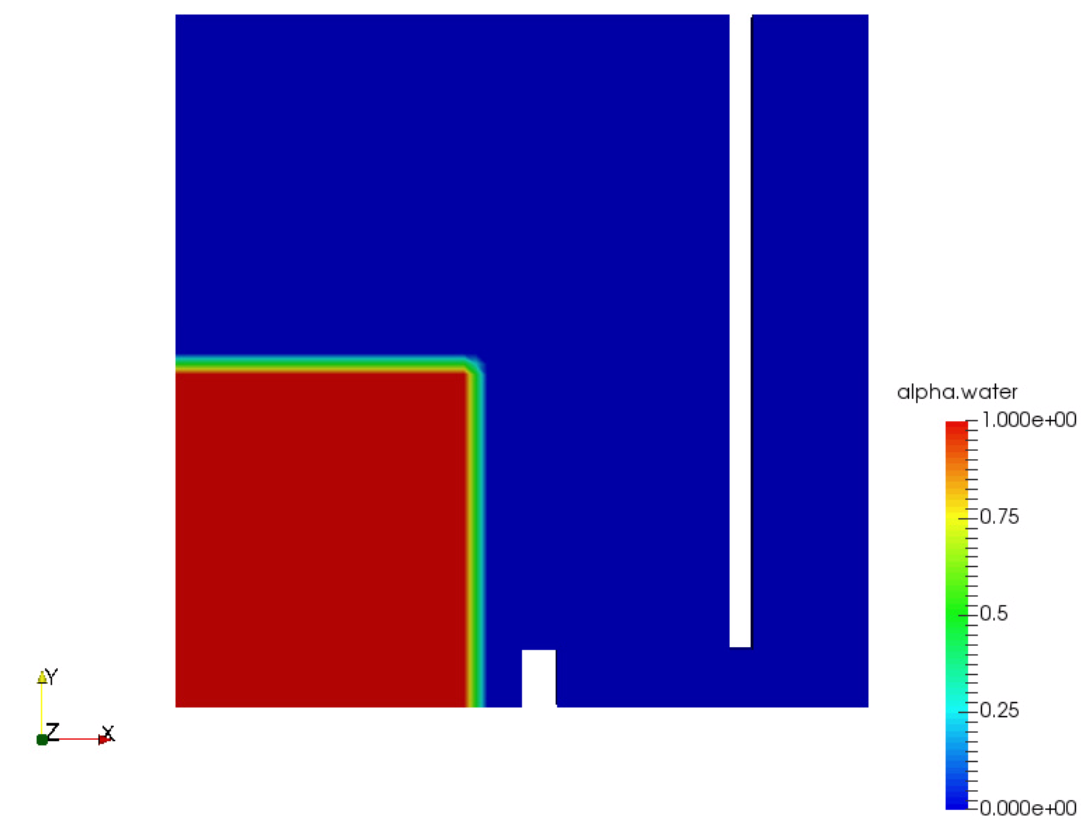
\includegraphics[width=0.7\linewidth]{sFdamBreakMod.png}
\caption{Condición inicial del agua}
\label{fig:sFdamBreakMod}
\end{figure}

\begin{figure}
\centering
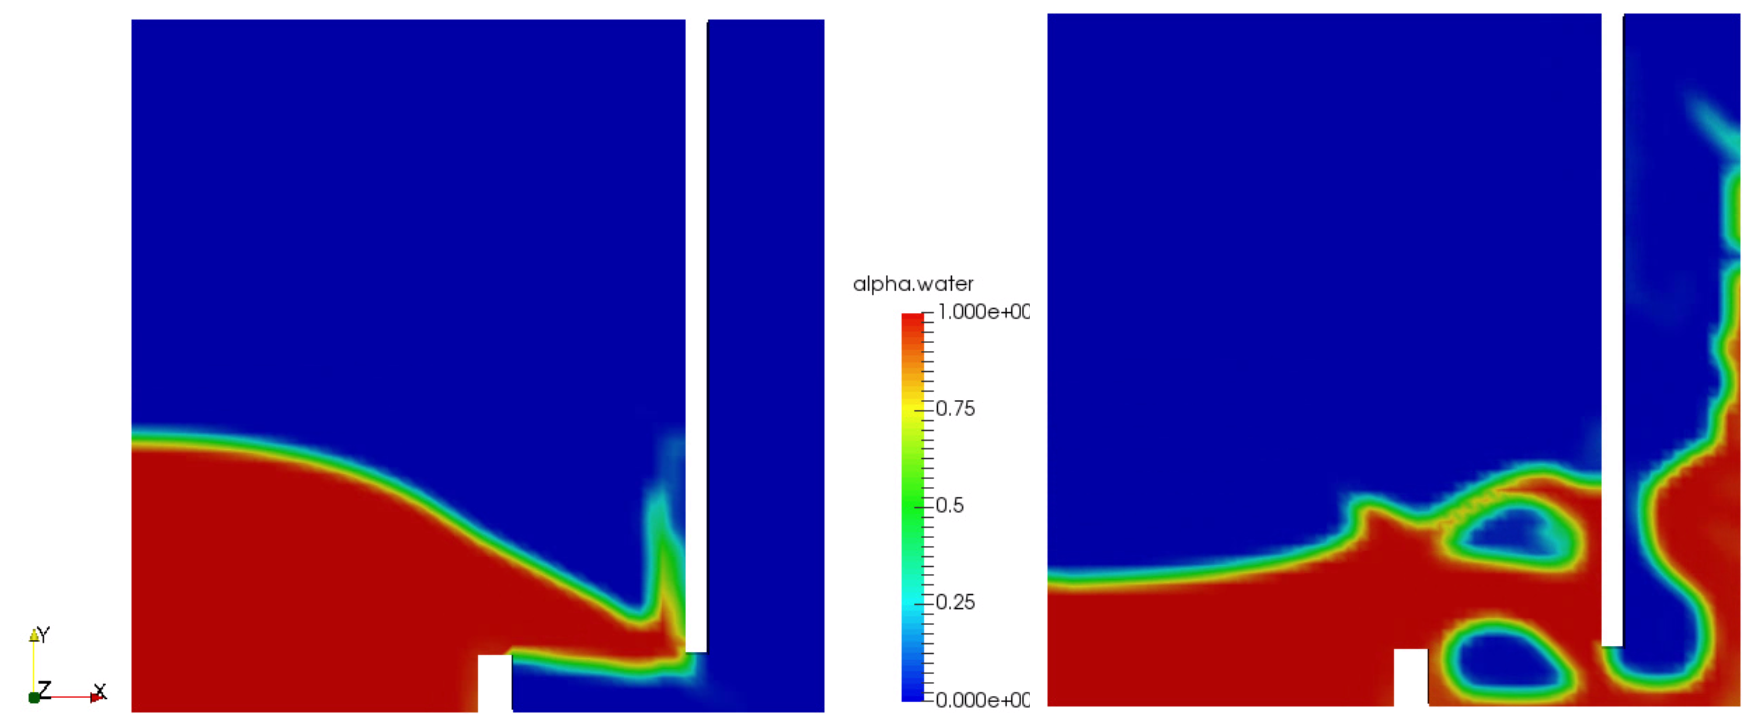
\includegraphics[width=\linewidth]{damBreakMod.png}
\caption{Imágenes del caso procesados gráficamente desde ParaView}
\label{fig:damBreakMod}
\end{figure}

\begin{enumerate}
\def\labelenumi{\arabic{enumi}.}
\item
  Desde la carpeta del caso, se ejecuta:
  \texttt{blockMesh\ \textgreater{}\ log.blockMesh}.
\item
  Comprobar la ausencia de errores en el modelo:
  \texttt{checkMesh\ \textbar{}\ tee\ log.checkMesh}.
\item
  Se ejecuta \texttt{paraFoam\ -block} para analizar el modelo generado
  y se vuelve a ejecutar \texttt{blockMesh}.
\item
  La utilidad \texttt{setFields} lee los campos del diccionario,
  recalculando y reescribiendo el archivo. Como ya se ha mencionado, se
  recomienda hacer una copia de seguridad de este archivo antes de
  ejecutar esta orden, debido a que el proceso anulará lo establecido:
  \texttt{cp\ 0/alpha.water.orig\ 0/alpha.water}. Ejecutar
  \texttt{paraFoam} para ver el resultado que se muestra en la imagen \autoref{fig:sFdamBreakMod}.


\item
  Procesado del caso mediante la orden:
  \texttt{interFoam\ \textbar{}\ tee\ log.interFoam} y visualizarlo con
  \texttt{paraFoam}, ver \autoref{fig:damBreakMod}.

\end{enumerate}

\subsection{damBreakSnappy}\label{header-n850}

Se parte por el caso base ``\emph{damBreak}'' y, para llevar a cabo el
proceso de generación del modelo con la utilidad \emph{snnappyHexMesh},
se tiene en cuenta el caso: \lstinline[style=bash]{$FOAM_run/incompressible/simpleFoam/motorBike}.

Además de las explicaciones contenidas en la guía
\cite{snappyHexMesh}.

\subsubsection{Definición del caso}\label{header-n855}

Por un lado se describe la malla base con \emph{blockMeshDict} (el
tamaño de las celdas deberá ser proximo a la unidad del ratio de aspecto
para un comportamiento óptimo de la solución) y los parámetros de
refinado se definen en \emph{snappyHexMeshDict}, utilidad que permite
generar el modelo a partir de un programa de CAD. Por tanto, para
ejecutar esta utilidad, se requiere la siguiente estructura básica:

\dirtree{%
.1 $<$case$>$.
.2 constant.
.3 triSurface.
.4 damBreakSnappy.stl.
.2 system.
.3 snappyHexMeshDict.
.3 blockMeshDict.
}

\begin{itemize}
\item
  Objetivos planteados:

  \begin{itemize}
  \item
    Implementar geometrías creadas desde un programa de CAD.
  \item
    Comprender cómo ejecutar un caso con la utilidad
    \texttt{snappyHexMesh} para generar la discretización del dominio de
    forma automatizada.
  \item
    Visualizar la altura de la SLL en la cámara.
  \end{itemize}
\item
  Definición de \emph{snappyHexMeshDict:}

  \begin{itemize}
  \item
    El refinado de las superficies se define de nivel (0 0), debido a
    que el caso de referencia que se está utilizando para realizar
    pruebas, ``\emph{damBreak}'', está definido en 2D, y si snappyHexMesh
    realiza divisiones en el eje Z, las simulaciones resultan en errores
    de cálculo. Es decir, como solución inicial, se incrementa la
    resolución desde \emph{blockMeshDict} y se utiliza
    \texttt{snappyHexMesh} únicamente para implementar la geometría
    generada en STL.
  \item
    El contenido del campo \texttt{features} se comenta, ya que en la
    prueba inicial no se ha utilizado la aplicación para extraer
    características.
  \item
    Para reducir el número de ficheros, la línea
    \lstinline[style=bash]{#include "meshQualityDict"} se ha sustituido por las
    opciones contenidas en:
    
    \lstinline[style=bash]{caseDicts/mesh/generation/meshQualityDict.cfg}.
  \end{itemize}
\item
  Condiciones iniciales:

  \begin{itemize}
  \item
    Se modifican los contornos de las variables principales contenidas
    en \lstinline[style=bash]{./0}, haciendo que correspondan con las
    definidas en el modelo.
  \end{itemize}
\item
  Preparación del fichero STL:

  \begin{itemize}
  \item
    El modelo que corresponde al espacio de simulación se ha creado
    mediante \emph{OpenSCAD} y exportado directamente en formato STL
    ascii.
  \item
    Como OpenSCAD no permite diferenciar regiones al exportar el sólido,
    se ha utilizado \emph{Blender}. Para trabajar con ficheros STL en
    Blender, se debe comprobar que el add-on correspondiente está
    activado, accediendo a las opciones de usuario (Ctrl+Alt+U) y
    buscando \texttt{Import-Export:\ STL\ format} en la pestaña
    \texttt{Add-ons}. Tras importar el fichero
    \lstinline[style=bash]{/of-dsgn/STL/damBreakMod.stl}, se puede trabajar con cada
    punto, vértice y cara. Las tareas de escalado/rotación/traslación
    del objeto es recomendable realizarlas en \emph{OpenSCAD}, pero se
    pueden utilizar filtros para mejorar el mallado resultante desde
    \emph{Blender}. Como se va a utilizar \texttt{snappyHexMesh}, se
    mantiene la estructura compuesta por el número mínimo de tetraedros.
  \end{itemize}
\end{itemize}

\begin{itemize}
\item
  Definición de contornos con Blender:

  \begin{itemize}
  \item
    Cambiar a \texttt{Edit\ Mode} y activar la selección por caras.
  \item
    Seleccionar todas las que correspondan al mismo contorno y darle a
    la tecla \texttt{p} y a \texttt{selection}, agrupando las caras
    seleccionadas en un nuevo objeto.

    \textbf{Nota}: se pueden seleccionar todas las caras que
    corresponden al mismo plano, pulsando \texttt{Ctrl+Alt+Shift+F} y
    botón derecho sobre una de las caras.
  \item
    Renombrar las regiones de forma apropiada (tanto los objetos como la
    estructura interna), en este caso se definen: \emph{allwall,
    atmosphere} y \emph{defaultFaces}.
  \item
    Se exporta cada objeto a un fichero STL, escogiendo el formato
    Ascii.
  \item
    Cambiar la primera y última línea de los ficheros nombrando
    debidamente cada contorno y unirlos en uno solo.
  \end{itemize}
\end{itemize}

\subsubsection{Ejecución del caso}\label{header-n927}

Se pueden ejecutar todas las tareas de forma automatizada mediante la
orden \lstinline[style=bash]{./RunCase damBreakSnappy} desde el directorio donde se
encuentra el \emph{script}. En este archivo se incluyen los pasos:

\begin{enumerate}
\def\labelenumi{\arabic{enumi}.}
\item
  Generar la geometría desde OpenSCAD y exportar a STL.
\item
  Utilizar Blender para definir las regiones (\emph{patches}) y exportar
  a un nuevo STL.
\item
  Se ejecuta \texttt{blockMesh}.
\item
  Se ejecuta \texttt{snappyHexMesh}.
\item
  Se mueven los ficheros correspondientes a la malla creada por
  blockMesh del directorio \lstinline[style=bash]{./constant} a un
  nuevo directorio \lstinline[style=bash]{./constant.bm}.
\item
  Se mueven los ficheros contenidos en la carpeta
  \lstinline[style=bash]{./0.002}, creados por snappyHexMesh, a la
  carpeta \lstinline[style=bash]{./constant}.
\item
  Se eliminan los directorios 0.001 y 0.002.
\item
  Se ejecuta \texttt{checkMesh} para comprobar que la malla es válidad.
\item
  Se copia 0/alpha.water.org a 0/alpha.water
\item
  Se ejecuta \texttt{setFields}. Si se muestra algún error, se debe
  comprobar que las regiones indicadas en
  \lstinline[style=bash]{./constant/polyMesh/boundary} coinciden con
  los condornos de los ficheros de la carpeta
  \lstinline[style=bash]{./0}.
\item
  Se ejecuta \texttt{interFoam}.
\item
  Se ejecuta paraFoam para visualizar los resultados, ver \autoref{fig:damBreakSnappy}.
\item
  Se borra \lstinline[style=bash]{0/alpha.water} al cerrar paraFoam.
\end{enumerate}

De la forma descrita, se pueden visualizar los pasos intermedios que se
crean con la orden \texttt{snappyHexMesh}, ayudando a su comprensión, ver \autoref{fig:snappy-damBreakSnappy}. 

No obstante, se puede añadir el argumento \texttt{-overwrite} al ejecutar
\texttt{snappyHexMesh}, para que se sobreescriba el contenido del
directorio \lstinline[style=bash]{./constant\textgreater} creado por
\texttt{blockMesh}, en vez de guardarse únicamente en la carpeta
\lstinline[style=bash]{./0.002}.

\begin{figure}[ht]
\centering
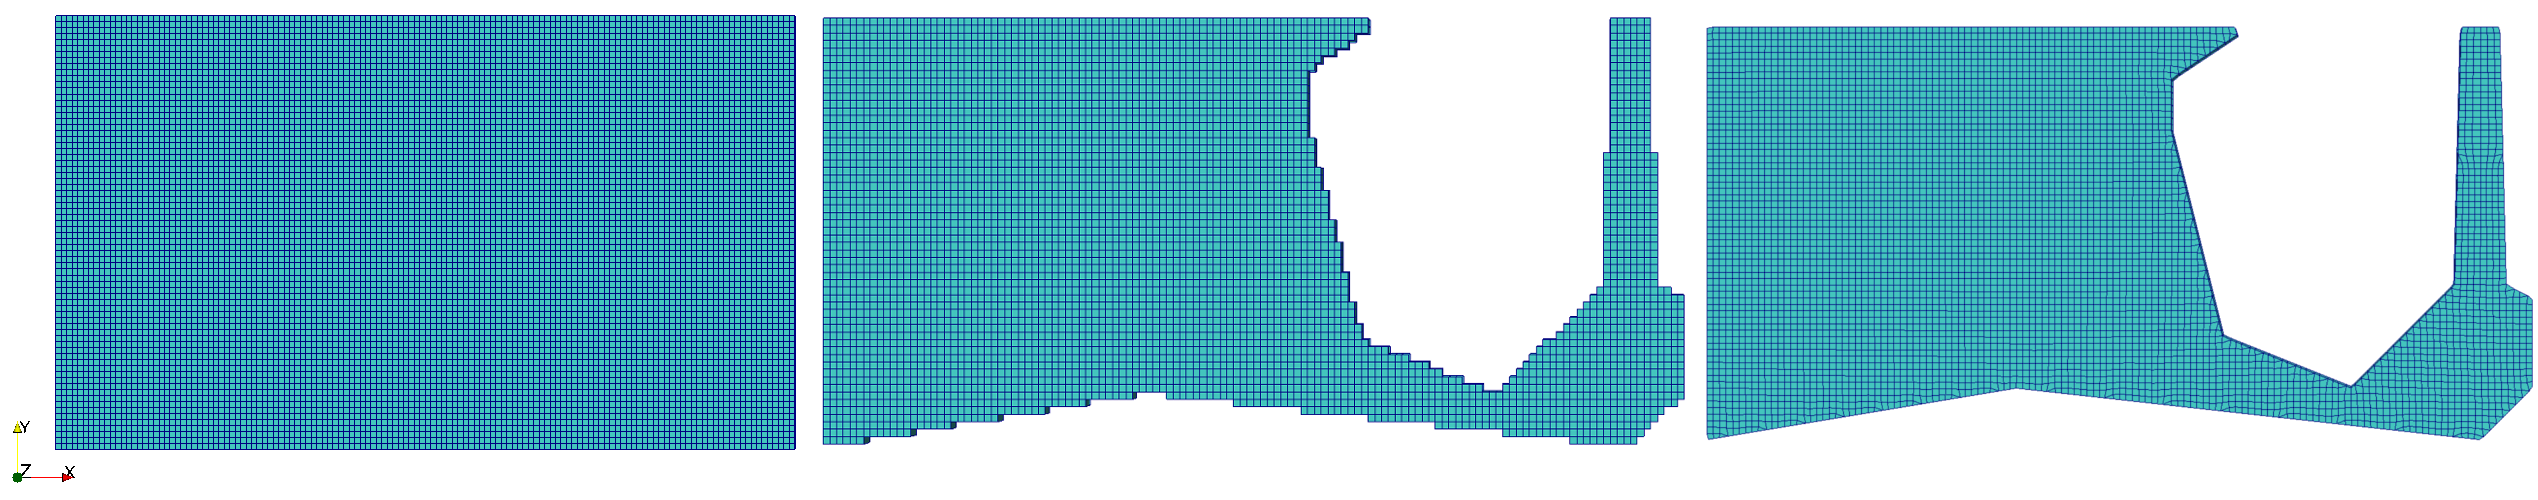
\includegraphics[width=\linewidth]{snappy-damBreakSnappy.png}
\caption{Proceso de generación del modelo}
\label{fig:snappy-damBreakSnappy}
\end{figure}

\begin{figure}[hb]
  \centering
  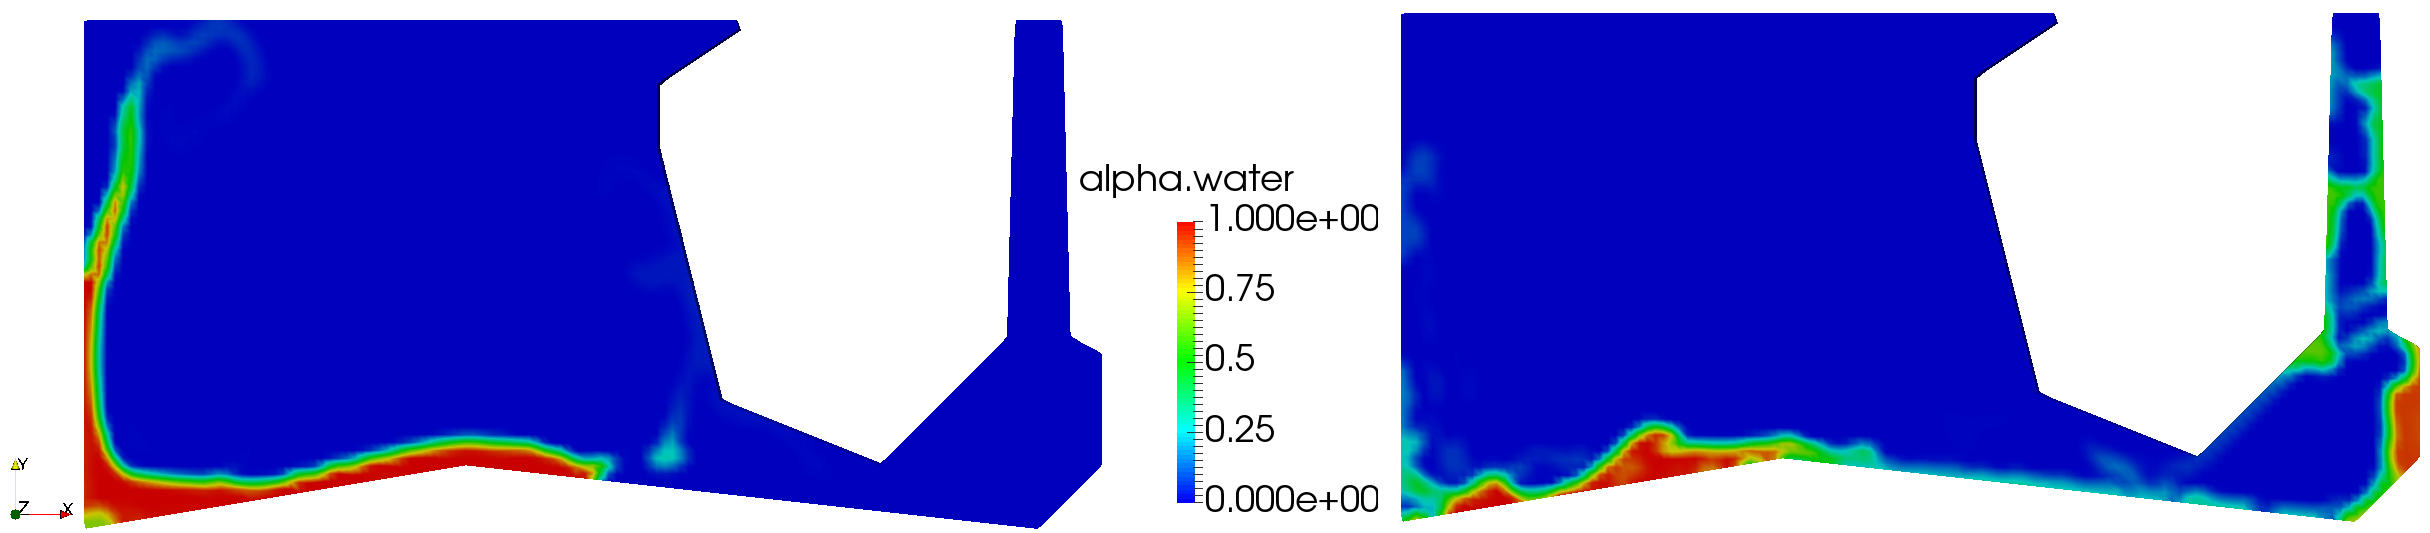
\includegraphics[width=\linewidth]{damBreakSnappy.png}
  \caption{Procesado de la solución desde ParaView}
  \label{fig:damBreakSnappy}
  \end{figure}

\subsection{damBreak3d}\label{header-n982}

En esta ocasión se aumenta la dimensión en el eje \emph{z} y se realizan
los cambios oportunos al caso base \emph{``damBreak''} para ejecutarlo en
3-D. Para ello, se consideran las pautas descritas en la referencia de Calum
Duglas \cite{calum}.

\subsubsection{Definición del caso}\label{header-n987}

\begin{itemize}
\item
  Objetivos planteados:

  \begin{itemize}
  \item
    Convertir un caso de 2-D a 3-D.
  \item
    Observar las direcciones que toma el flujo de agua en las tres
    direcciones.
  \end{itemize}
\item
  Definición del modelo:

  \begin{itemize}
  \item
    Definir una anchura de \(z=2*0,146=0,292 m\) (donde 0,146
    corresponde al valor definido en \texttt{convertToMeters}, en
    \emph{blockMeshDict} las dimensiones definidas por cada vértice son
    sin escala, se multiplican por este número para convertirlas a
    metros).
  \item
    Descomponer el dominio de manera proporcional al eje \emph{x} e
    \emph{y}, luego el número de celdas correspondiente al eje \emph{z}
    se establece a 8.
  \item
    Definir el contorno \emph{``frontback''} como pared (\emph{wall}),
    para obtener la solución, también, en el eje \emph{z}.
  \end{itemize}
\item
  Condiciones iniciales

  \begin{itemize}
  \item
    El agua se define sin ocupar todo el ancho (en \emph{z}) para
    analizar cómo se comporta en sus tres ejes. Los valores mínimo y
    máximo que determinan el prisma correspondiente al volumen ocupado
    por agua son: \lstinline[style=bash]{box (0 0 0) (0.1461 0.292 0.15);}
  \end{itemize}
\item
  Condiciones de contorno:

  \begin{itemize}
  \item
    Modificar el campo correspondiente al contorno \emph{frontback} de
    cada variable principal de forma afin a la descripción de un
    contorno de las mismas características (p.e. \emph{leftWall}).
  \end{itemize}
\end{itemize}

\subsubsection{Ejecución del caso}\label{header-n1027}

Para ejecutar el caso se siguen los pasos básicos:

\begin{figure}
\centering
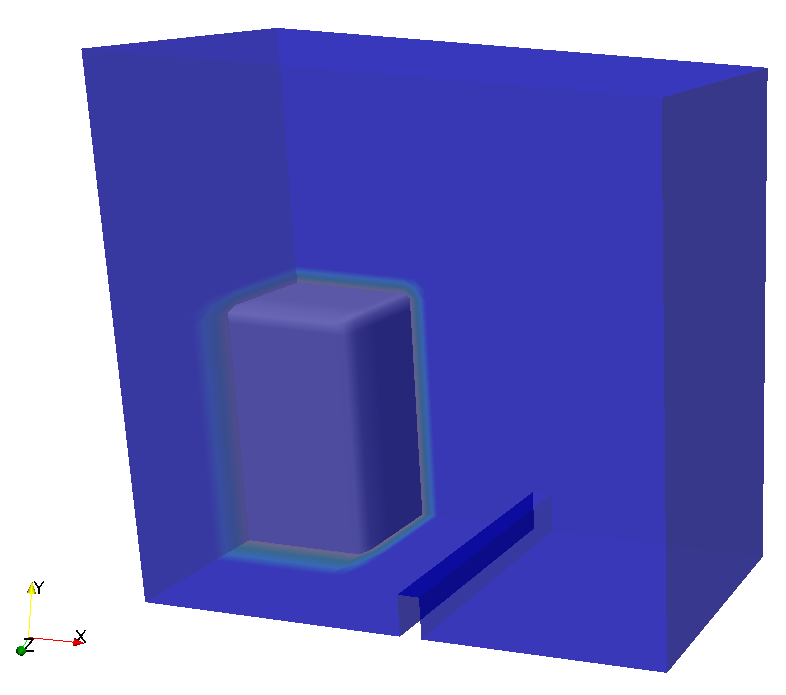
\includegraphics[scale=0.3]{sFdamBreak3d.png}
\caption[Condición inicial del volumen del agua]{Visualización desde ParaView de la condición inicial del volumen del agua}
\label{fig:sFdamBreak3d}
\end{figure}

\begin{figure}
\centering
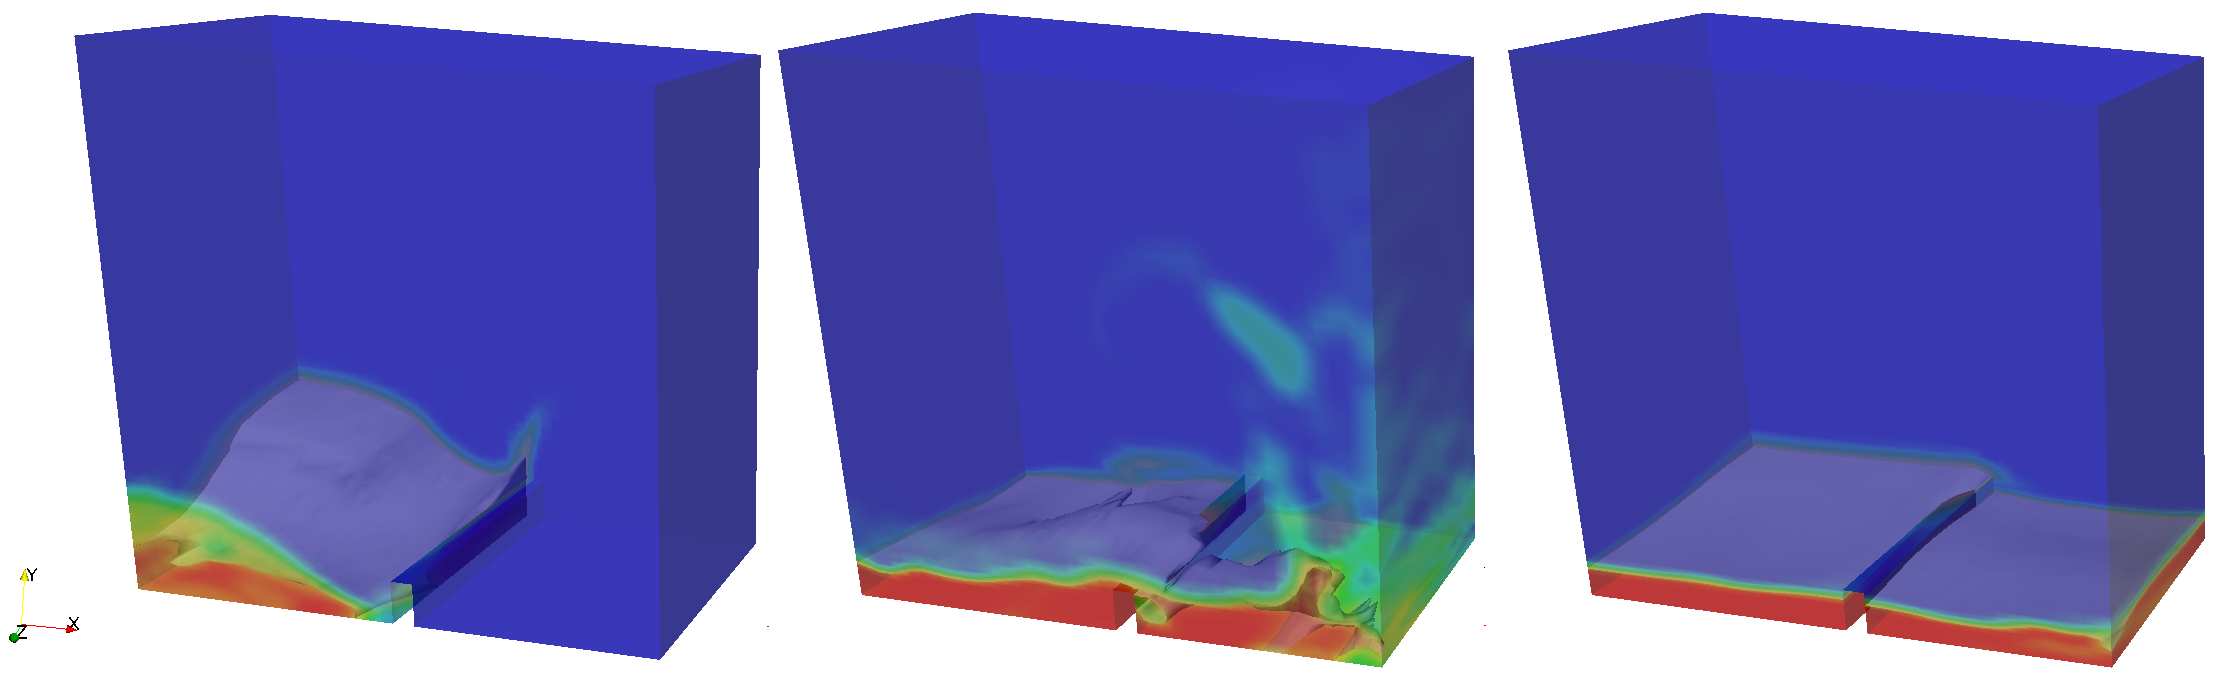
\includegraphics[width=\linewidth]{damBreak3d.png}
\caption{Imágenes de la solución visualizada desde ParaView}
\label{fig:damBreak3d}
\end{figure}

\begin{enumerate}
\def\labelenumi{\arabic{enumi}.}
\item
  Generar el modelo con la orden:
  \lstinline[style=bash]{blockMesh > log.blockMesh}.
\item
  Comprobar la ausencia de errores:
  \lstinline[style=bash]{checkMesh > log.checkMesh}.
\item
  Comprobar que existen los archivos \emph{alpha.water} y
  \emph{alpha.water.orig}, ejecutar:
  \lstinline[style=bash]{setFields > log.setFields}.
  De esta forma se define el volumen de agua en las celdas del dominio, \autoref{fig:sFdamBreak3d}.
\item
  Procesar el caso con la orden:
  \lstinline[style=bash]{interFoam > log.interFoam}.
\item
  Visualizar el resultado: ejecutando \lstinline[style=bash]{paraFoam}.  
  Asimismo desde ParaView definir los parámetros de visualización \autoref{fig:damBreak3d}.
\end{enumerate}
